%%%%%%%%%%%%%%%%%%%%%%%%%%%%%%%%%%%%%%%%% 
% Beamer Presentation LaTeX Template Version 1.0 (10/11/12)
% 
% This template has been downloaded from:
% http://www.LaTeXTemplates.com
% 
% License: CC BY-NC-SA 3.0
% (http://creativecommons.org/licenses/by-nc-sa/3.0/)
% 
%%%%%%%%%%%%%%%%%%%%%%%%%%%%%%%%%%%%%%%%% 

% ----------------------------------------------------------------------------------------
% PACKAGES AND THEMES
% ----------------------------------------------------------------------------------------

\documentclass{beamer}

\mode<presentation> {

  % The Beamer class comes with a number of default slide themes
  % which change the colors and layouts of slides. Below this is a
  % list
  % of all the themes, uncomment each in turn to see what they look
  % like.

  % \usetheme{default}
  % \usetheme{AnnArbor}
  % \usetheme{Antibes}
  % \usetheme{Bergen}
  % \usetheme{Berkeley}
  % \usetheme{Berlin}
  % \usetheme{Boadilla}
  % \usetheme{CambridgeUS}
  % \usetheme{Copenhagen}
  % \usetheme{Darmstadt}
  % \usetheme{Dresden}
  % \usetheme{Frankfurt}
  \usetheme{Goettingen}
  % \usetheme{Hannover}
  % \usetheme{Ilmenau}
  % \usetheme{JuanLesPins}
  % \usetheme{Luebeck}
  % \usetheme{Madrid}
  % \usetheme{Malmoe}
  % \usetheme{Marburg}
  % \usetheme{Montpellier}
  % \usetheme{PaloAlto}
  % \usetheme{Pittsburgh}
  % \usetheme{Rochester}
  % \usetheme{Singapore}
  % \usetheme{Szeged}
  % \usetheme{Warsaw}

  % As well as themes, the Beamer class has a number of color themes
  % for any slide theme. Uncomment each of these in turn to see how it
  % changes the colors of your current slide theme.

  % \usecolortheme{albatross}
  % \usecolortheme{beaver}
  % \usecolortheme{beetle}
  % \usecolortheme{crane}
  % \usecolortheme{dolphin}
  % \usecolortheme{dove}
  % \usecolortheme{fly}
  % \usecolortheme{lily}
  % \usecolortheme{orchid}
  % \usecolortheme{rose}
  % \usecolortheme{seagull}
  % \usecolortheme{seahorse}
  % \usecolortheme{whale}
  % \usecolortheme{wolverine}

  % \setbeamertemplate{footline} % To remove the footer line in all slides uncomment this line
  \setbeamertemplate{footline}[page
  number] % To replace the footer line in all slides with a simple slide count uncomment this line

  % \setbeamertemplate{navigation
  % symbols}{} % To remove the navigation symbols from the bottom of all slides uncomment this line
}

\usepackage{graphicx} % Allows including images
\usepackage{booktabs} % Allows the use of \toprule, \midrule and \bottomrule in tables
\usepackage[german]{babel} % Required to compile in Windows
\usepackage[latin1]{inputenc} \usepackage{caption}
\usepackage{subcaption}
% \usepackage{physics}
\usepackage{mathtools} \usepackage{natbib} \usepackage[T1]{fontenc}


\AtBeginSection[]{
  \begin{frame}
    \vfill \centering
    \begin{beamercolorbox}[sep = 8pt, center, shadow = true, rounded =
      true]{title}
      \usebeamerfont{title}\insertsectionhead\par%
    \end{beamercolorbox}
    \vfill
  \end{frame}
}

% ----------------------------------------------------------------------------------------
% TITLE PAGE
% ----------------------------------------------------------------------------------------

\title[]{Projekt 1a:
  Abschlusspr�sentation} % The short title appears at the bottom of every slide, the full title is only on the title page

\author{Isabell Albrecht, Erik Engelhardt, Oliver Kochan, Florian
  Steffens} % Your name
\institute[HAW] % Your institution as it will appear on the bottom of every slide, may be shorthand to save space
{ Hochschule f�r angewandte Wissenschaften -- Hamburg
  \\ % Your institution for the title page
  \medskip
  % \textit{erik.engelhardt@haw-hamburg.de,
  % hier@email.eintragen} % Your email address
}

\date{\today} % Date, can be changed to a custom date

\begin{document}

\begin{frame}
  \titlepage % Print the title page as the first slide
\end{frame}

\section{Einleitung}
% - Gruppenmitglieder vorstellen - welches Projekt bearbeiten wir
% (Bild)
\begin{frame}
  \frametitle{Wetterstation - Projekt 1a}
  \begin{figure}
    \centering
    \begin{minipage}[t]{0.45\linewidth}
      \centering
      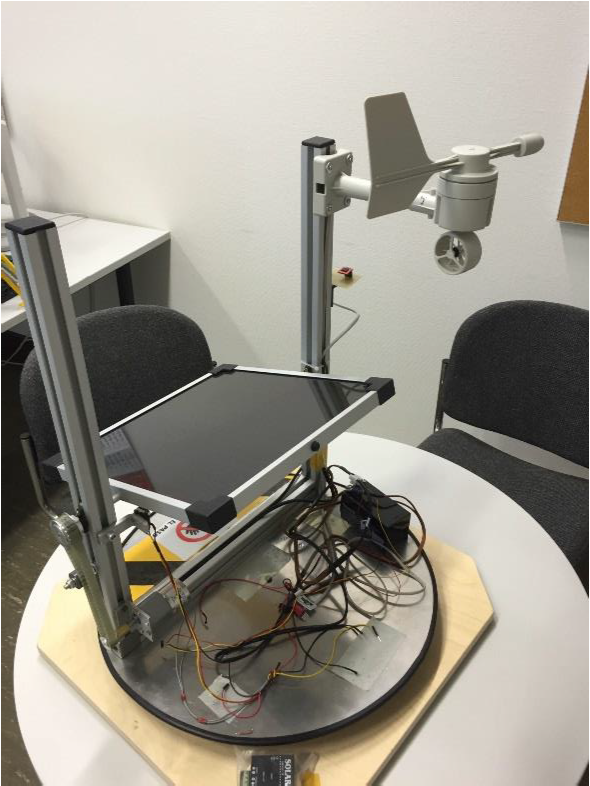
\includegraphics[width=\linewidth]{img/Wetterstation_1.png}
    \end{minipage}% <- sonst wird hier ein Leerzeichen eingefügt
    \hfill
    \begin{minipage}[t]{0.45\linewidth}
      \centering
      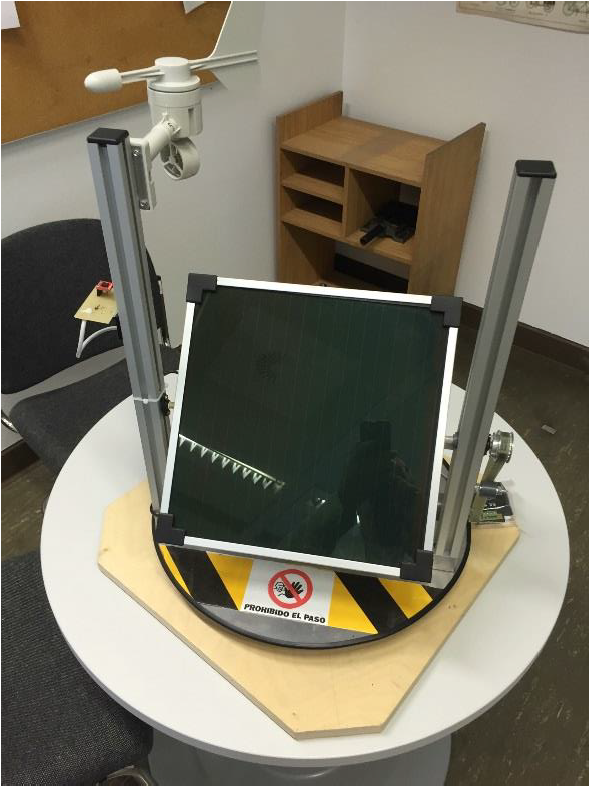
\includegraphics[width=\linewidth]{img/Wetterstation_2.png}
    \end{minipage}
  \end{figure}
  % \emph{Diese Wetterstation wird sehr gut.}
\end{frame}

\begin{frame}[allowframebreaks]
  % \frametitle{Gliederung} % Table of contents slide, comment this block out to remove it
  \tableofcontents % Throughout your presentation, if you choose to use \section{} and \subsection{} commands, these will automatically be printed on this slide as an overview of your presentation
\end{frame}
% ----------------------------------------------------------------------------------------
% PRESENTATION SLIDES NEW
% ----------------------------------------------------------------------------------------

\section{Live-Demo}

\section{Nutzeroberfl�che}

\begin{frame}
  \frametitle{Funktionen}
  \begin{figure}[H]
    \centering
    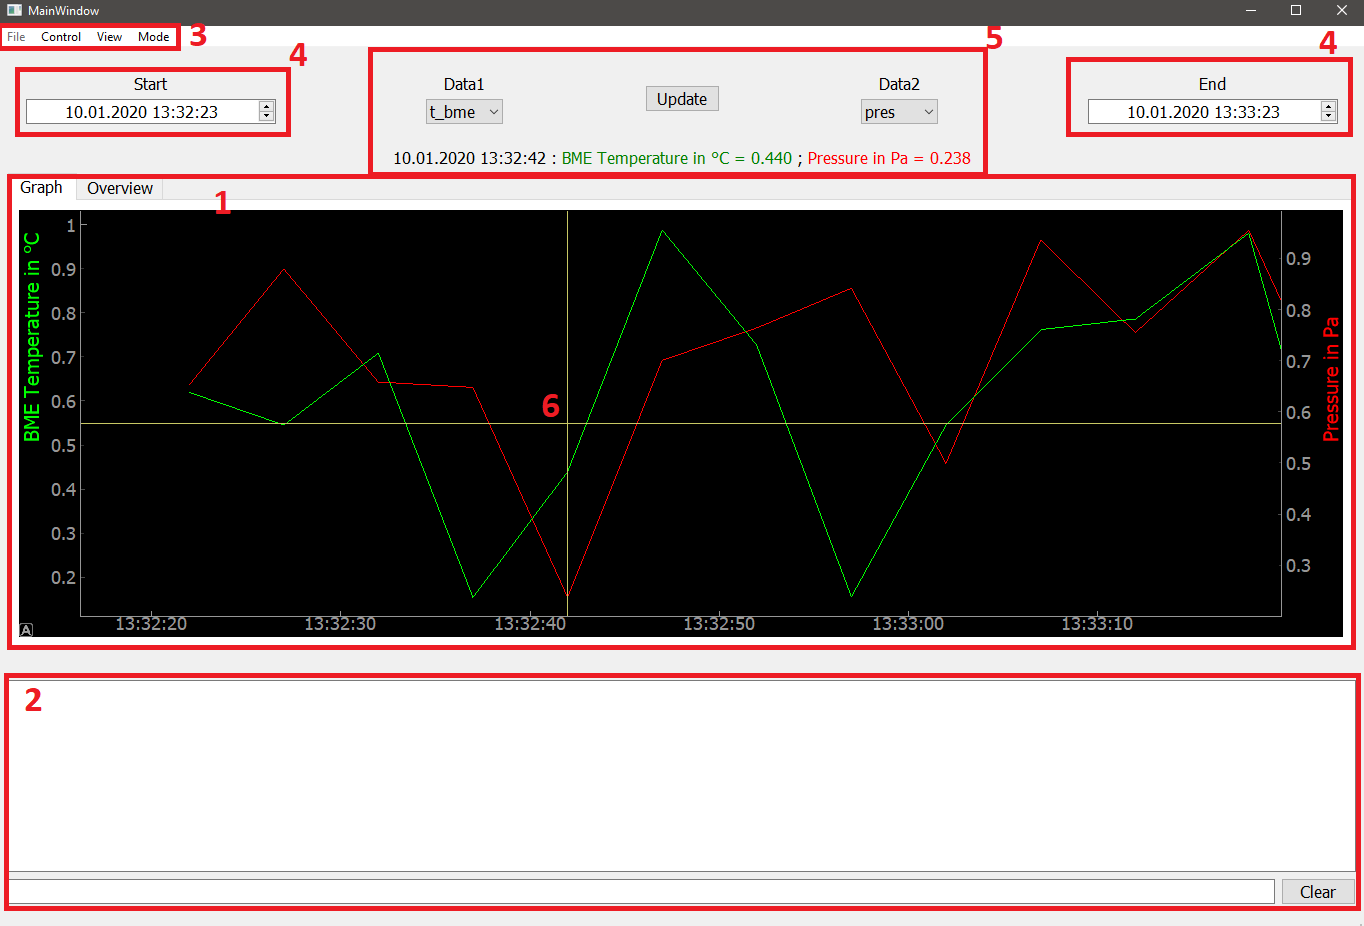
\includegraphics[width=\textwidth]{./img/ui_simulated_graph}
  \end{figure}
\end{frame}
\begin{frame}
  \frametitle{Funktionen}
  \begin{figure}[H]
  \centering
  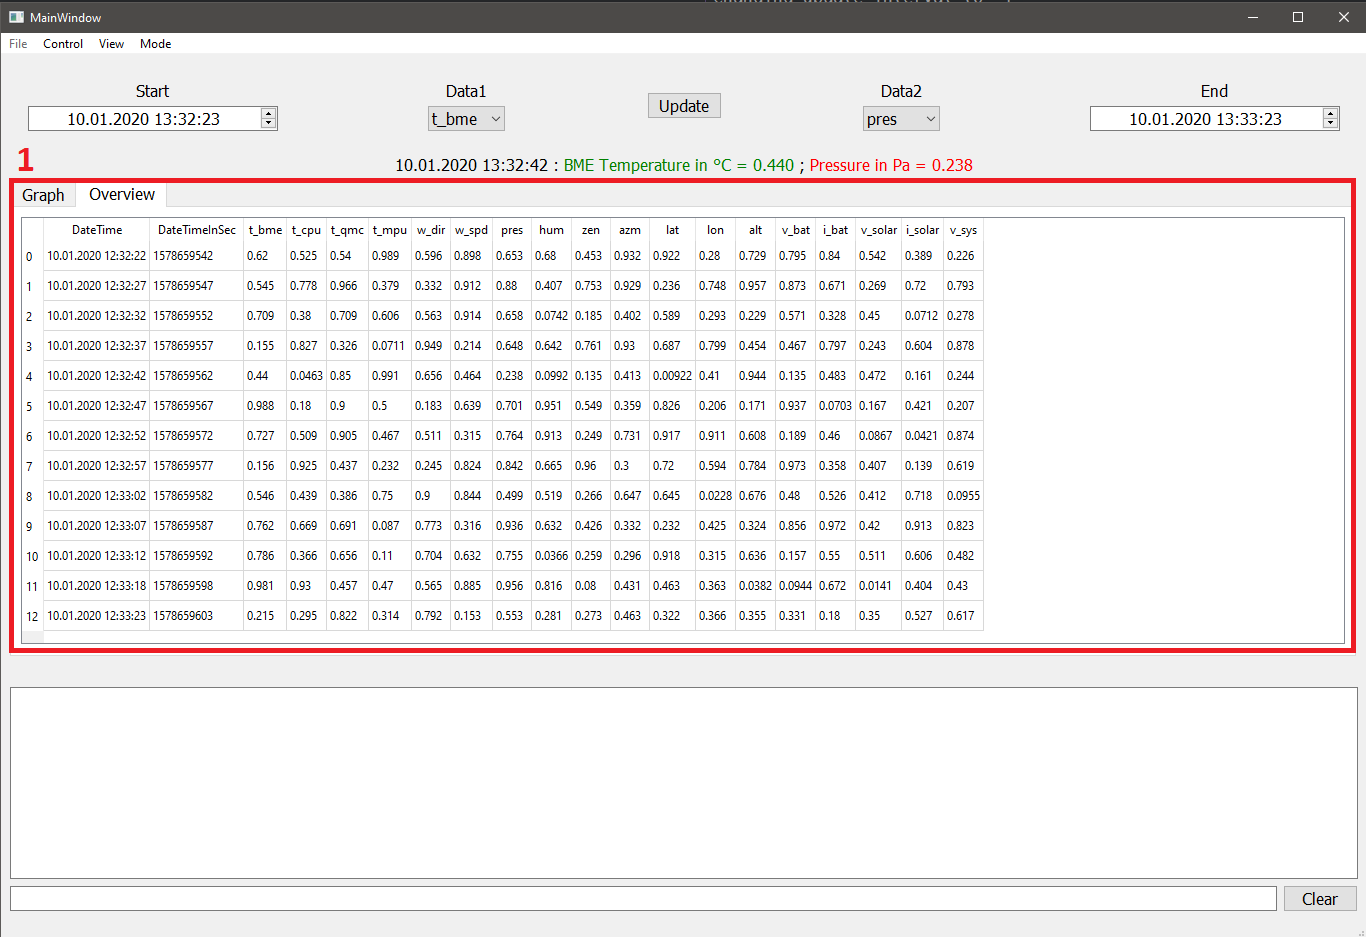
\includegraphics[width=\textwidth]{./img/ui_simulated_table}
\end{figure}
\end{frame}
\begin{frame}
  \frametitle{Geplante Funktionen}
  \begin{itemize}
  \item Speichern und Laden von Messdaten auf dem Computer
  \item Auslagerung der Kommunikation mit der Wetterstation in einen eigenen Task
  \item Einstellen der Kommunikationsschnittstelle �ber die Benutzeroberfl�che
  \item Benutzerdefinierte �nderung der Position und des Datums / der Zeit �ber ein Bedienelement
  \end{itemize}
\end{frame}
\begin{frame}
  \frametitle{Model-View-Controller}
  \begin{figure}[H]
    \centering 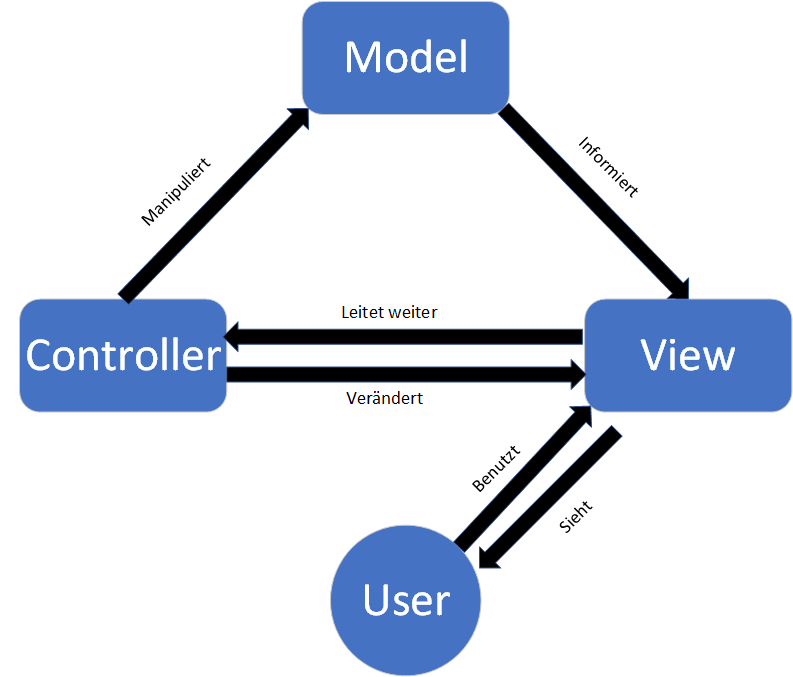
\includegraphics[width=.7\textwidth]{./img/MVC.png}
  \end{figure}
\end{frame}

\begin{frame}
  \frametitle{Verwendete Python-Packages}
  \begin{itemize}
  \item PyQt5: Als Framework f�r die Oberfl�che.
  \item pyqtgraph: F�r die graphische Darstellung der Messdaten.
  \item serial: F�r die serielle Kommunikation, �ber Bluetooth, mit
    der Wetterstation.
  \item pandas: F�r die Strukturierung der Messdaten.
  \item numpy: F�r das Erstellen von Testdaten.
  \end{itemize}

\end{frame}

\section{3D gedruckte Komponenten}
\begin{frame}
  \frametitle{Nebengeh�use}
  \begin{itemize}
  \item Sichere Unterbringung von GPS-Modul, Kompass-Modul, und Neigungssensor
  \item Befestigung an der Wetterstation mittels Schrauben
  \item Befestigung des Deckels mittels Steckverbindung und Kabelbindern
  \end{itemize}
  \begin{figure}[H]
    \centering 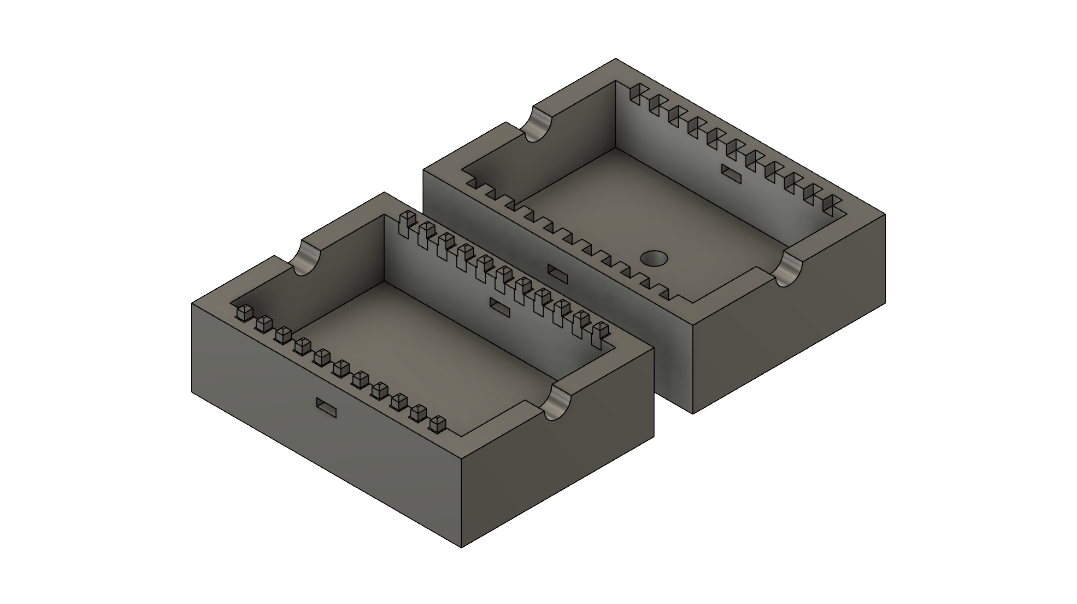
\includegraphics[width=.7\textwidth]{./img/ST_Halterv5}
  \end{figure}
\end{frame}
\begin{frame}
  \begin{itemize}
  \item F�r die Verbindung des Masts (Anemometer und Windfahne) mit der Wetterstation
  \item Befestigung an de Wetterstation mittels Steckverbindung
  \item Verbindung mit dem Mast �ber Steckverbindung und optionale Schraubverbindung
  \end{itemize}
  \frametitle{Adapter}
  \begin{figure}[H]
    \centering 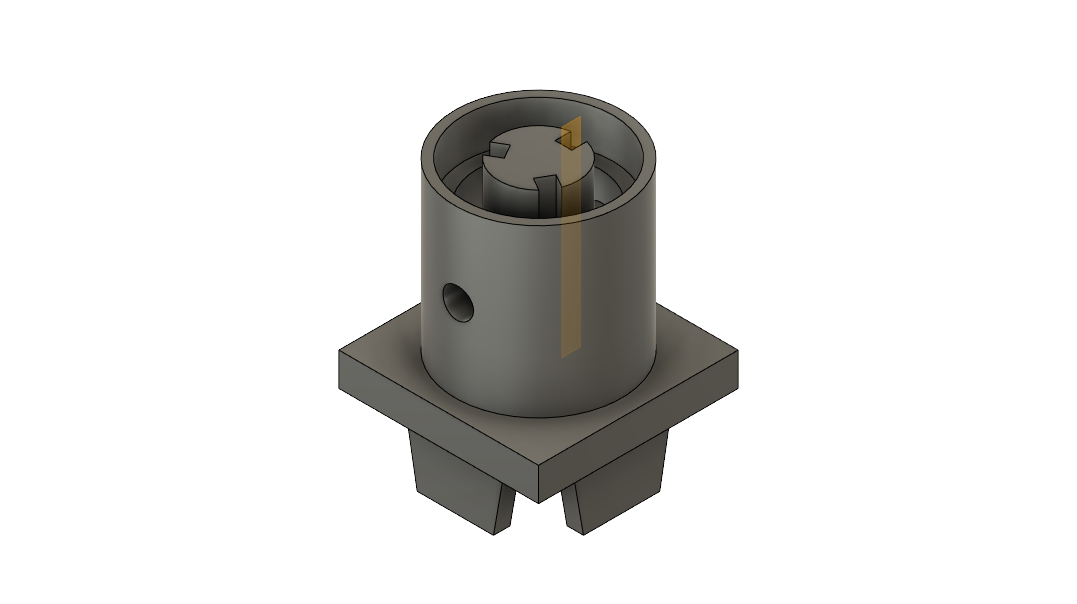
\includegraphics[width=.7\textwidth]{./img/ST_Adapterv4}
  \end{figure}
\end{frame}
\begin{frame}
  \frametitle{Hauptgeh�use}
  \begin{itemize}
  \item F�r die Unterbringung des Mikrocontrollers, der Spannungsversorgung und des Motortreibers
  \item Befestigung an der Wetterstation mittels Klebverbindung
  \item Befestigung des Deckels mittels Steckverbindung und optionalen Kabelbindern
  \end{itemize}
  \begin{figure}[H]
    \centering
    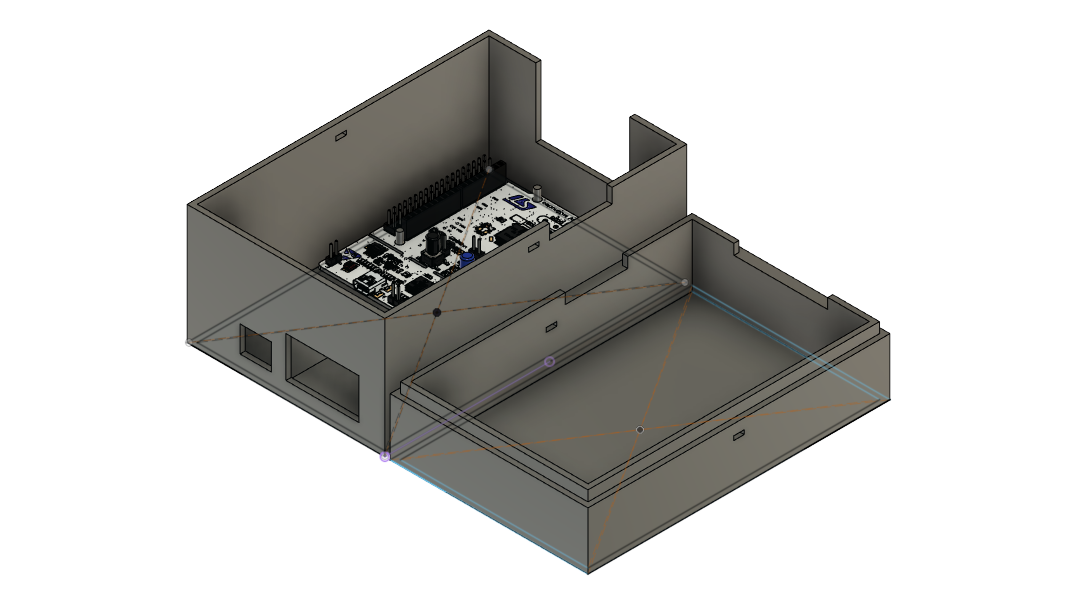
\includegraphics[width=.7\textwidth]{./img/ST_MainBodyv13}
  \end{figure}
\end{frame}
\begin{frame}
  \frametitle{Allgemeines}
  \begin{itemize}
  \item Entwurf der Komponenten in Autocad Fusion 360
  \item Material der Komponenten: PLA
  \item Druck mit 2-3 Au�enlagen und 10\%-20\% Infill
  \end{itemize}
\begin{figure}[H]
  \centering
  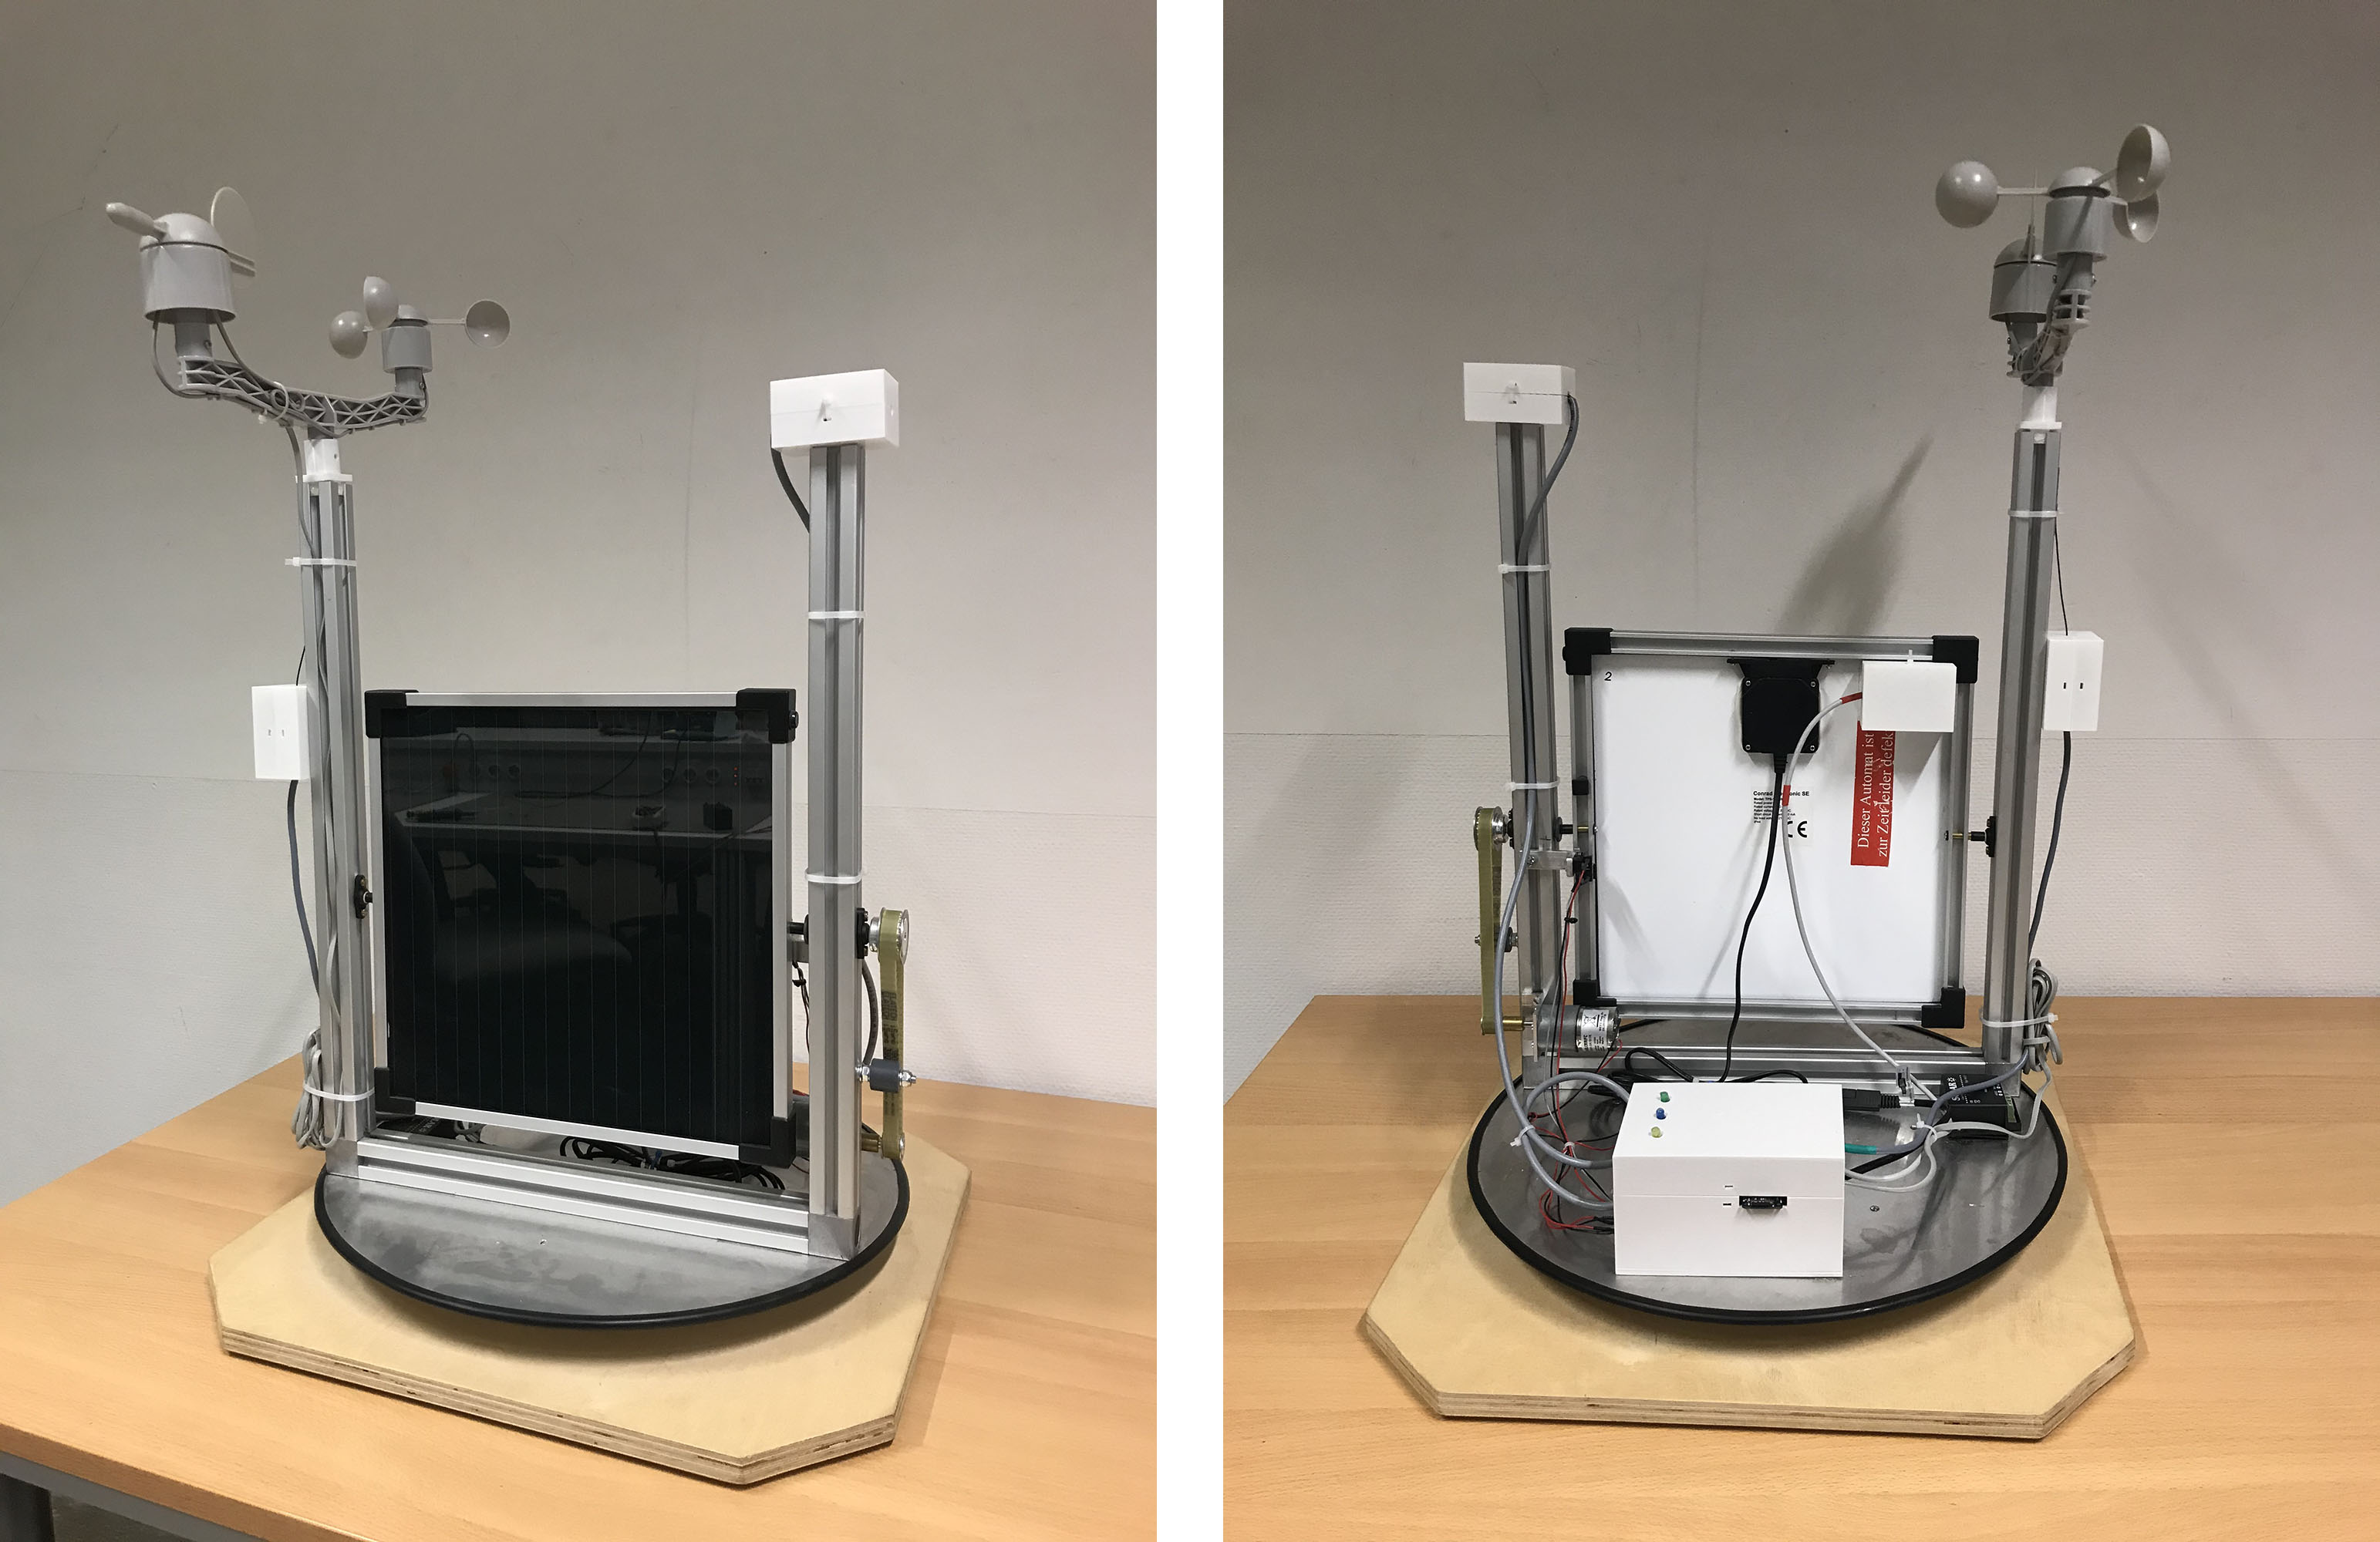
\includegraphics[width=0.7\textwidth]{./img/Wetterstaion_fertig1.jpg}
\end{figure}
  
\end{frame}
\section{Fazit}




% ----------------------------------------------------------------------------------------
% PRESENTATION SLIDES OLD
% ----------------------------------------------------------------------------------------

% \section{Software}
% % - zusammenfassen der Puntke aus Vorlage - eingrenzung Messbereiche
% \subsection{Fertig}
% \begin{frame}
%   \frametitle{Software - Fertig}
%   \begin{itemize}
%   \item \emph{Grundger�st}
%   \item \emph{Ansteuerung I2C, SPI, UART, ADC, RTC}
%   \item \emph{Einlesen und Umrechnen der Sensordaten}
%   \item \emph{Lageregelung}
%   \item \emph{Auswertung NMEA-Sentences vom GPS-Modul}
%   \item \emph{Berechnung von Azimut und Elevation}
%   \item \emph{Kommunikation über Bluetooth}
%   \item \emph{Externe Bibliothek f�r FAT32-Dateisystem}
%   \item \emph{Energiesparma�nahmen}
%   \end{itemize}
% \end{frame}

% \begin{frame}
%   \frametitle{Berechnung der Sonnenposition}
%   \begin{itemize}
%   \item Berechnung von Zenith und Azimut
%   \item Implementierung nach \citet[]{Roderick1992}
%   \end{itemize}
%   \begin{figure}[hbtp]
%     \centering
%     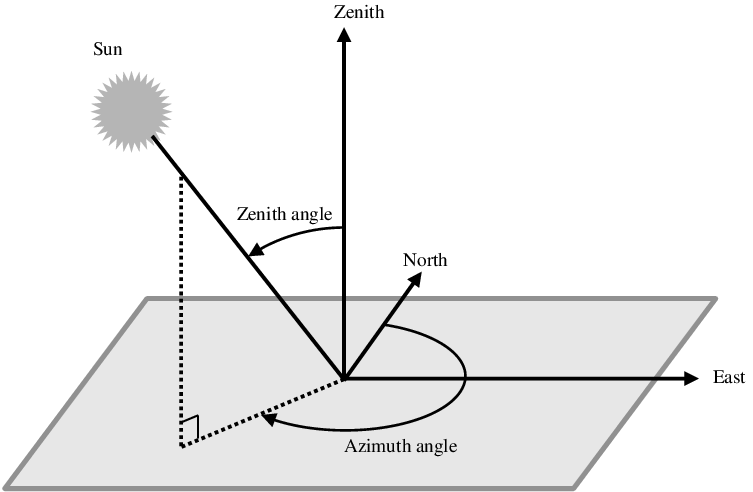
\includegraphics[width=0.6\textwidth]{./img/Representation-of-azimuth-and-zenith-angles.png}
%     \caption{Beschreibung der Sonnenposition durch Zenith und
%     Azimut~\cite[]{Nou2016}}\label{fig:zen_azi}
%   \end{figure}
% \end{frame}
% \begin{frame}
%   \frametitle{Berechnung der Sonnenposition (Beispiel)}
%   \begin{itemize}
%   \item Hamburg, 26.11.2019, 9:30h
%   \item Zenith = 81.1�
%   \item Azimuth = 143.3�
%   \end{itemize}
%   \begin{figure}[hbtp]
%     \centering
%     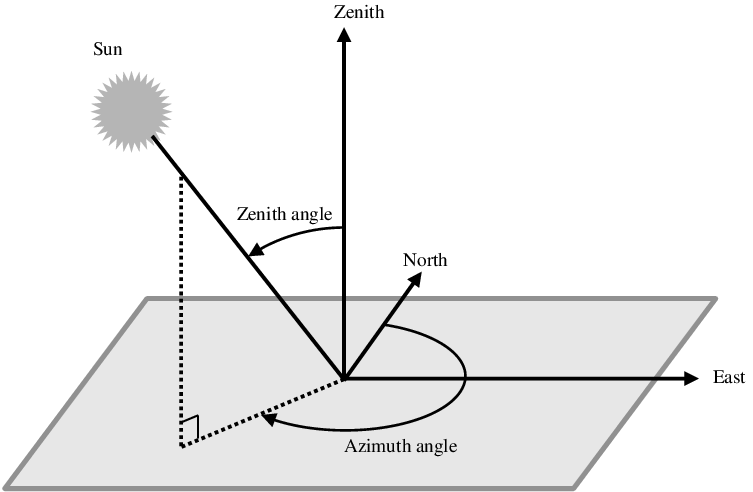
\includegraphics[width=0.6\textwidth]{./img/Representation-of-azimuth-and-zenith-angles.png}
%     \caption{Beschreibung der Sonnenposition durch Zenith und
%     Azimut~\cite[]{Nou2016}}\label{fig:zen_azi}
%   \end{figure}
% \end{frame}
% \subsection{Ausstehend}
% \begin{frame}
%   \frametitle{Software - Ausstehend}
%   \begin{itemize}
%   \item \emph{Zeitgesteuerte Nachf�hrung des Panels}
%   \item \emph{Bluetooth: AT command set; Demo-Mode}
%   \item \emph{Visualisierungssoftware auf einem PC}
%   \item \emph{Speichern der Sensordaten auf der SD-Karte}
%   \end{itemize}
% \end{frame}

% % \end{frame}
% \section{Elektronik}
% % - Sensoren kurz vorstellen und Bezug auf Anforderungen nehmen
% \begin{frame}
%   \frametitle{Elektronik - Fertig}
%   \subsection{Fertig}
        
%   \begin{itemize}
%   \item \emph{Spannungsversorgung}
%   \item \emph{Schaltplan}
%   \item \emph{Platinenlayout}
%   \item \emph{Test der Motoren}
%   \end{itemize}
% \end{frame}

% \begin{frame}
%   \frametitle{Elektronik - Ausstehend}
%   \subsection{Ausstehend}
%   \begin{itemize}
%   \item \emph{Aufbau der Platine}
%   \item \emph{Verkabelung der Sensoren}
%   \item \emph{Kabelmanagement}
%   \end{itemize}
% \end{frame}
    
% \section{Aufbau}
% \begin{frame}
%   \frametitle{Aufbaue - Fertig}
%   \subsection{Fertig}
%   \begin{itemize}
%   \item \emph{Planung}
%   \item \emph{Stabilit�t des Solarmoduls}
%   \item \emph{3D-Druck - Halterung f�r Sensoren}
%   \end{itemize}
%   \begin{figure}[hbtp]
%     \centering
%     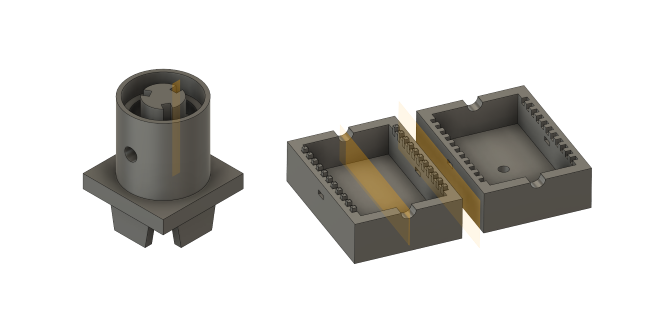
\includegraphics[width=0.8\textwidth]{./img/druck.png}
%     \caption{Adapter und Halter f�r die Sensoren}
%   \end{figure}
% \end{frame}

% \begin{frame}
%   \frametitle{Aufbau - Ausstehend}
%   \subsection{Ausstehend}
%   \begin{itemize}
%   \item \emph{Montage - Halterungen}
%   \item \emph{Montage - Sensoren}
%   \item \emph{Montage - Kabel}
%   \item \emph{Montage - Geh�use (Platine)}
%   \item \emph{Montage - Spannungsversorgung}
%   \item \emph{3D-Druck - Geh�use}
%   \end{itemize}
% \end{frame}

% \section{Zeitplan}
% % - groben Zeitplan vorstellen (Diagramm)

% \begin{frame}
%   \frametitle{Zeitplan}
%   \begin{itemize}
%   \item \emph{Planung ist vollst�ndig abgeschlossen}
%   \item \emph{Fortf�hrung nach Ankunft der Platine}
%   \item \emph{Dokumentation} %wird Montag eingereicht
%   \end{itemize}
% \end{frame}
\begin{frame}[allowframebreaks]
  \frametitle{Literatur- und Quellenverzeichnis}
  \bibliographystyle{plainnat} \bibliography{literature}
\end{frame}

% ------------------------------------------------
% ----------------------------------------------------------------------------------------

\end{document}
%%% Local Variables:
%%% mode: latex
%%% TeX-master: t
%%% End:
